\documentclass[a4paper,12pt]{article}
\usepackage{graphicx}
\usepackage{float}
\begin{document}

\graphicspath{{images/}}
\newcommand{\ie}{\textit{i}.\textit{e}., }
\newcommand{\eg}{\textit{e}.\textit{g}. }

\title{Different types of RAM}
\date{}
\author{Masih Ahmed, 18117056, Btech 2nd year CSE}
\maketitle
RAM stands for Random Access Memory, and it gives computers the virtual space needed to manage information and solve problems in the moment. It is a part of computer's main memory which is accessible by the CPU and is capable of performing read and write operations. RAM is volatile in nature, that is, once power is cut off, information is lost. It is used to store the data that is currently being processed by the CPU.
The different types of RAM are: 

\section{SRAM - Static RAM}
SRAM requires a constant power flow in order to function. Because of the continuous power, SRAM doesn’t need to be ‘refreshed’ to remember the data being stored. This is why SRAM is called ‘static’ – no change or action (\eg refreshing) is needed to keep data intact. The word line is activated by the address input to the address decoder. As a consequence, the transistors are in active state, and read and write operations are passed through the bit lines. 
\\
\\The advantages of using SRAM (vs. DRAM) are lower power consumption and faster access speeds. 
\\The disadvantages of using SRAM (vs. DRAM) are lesser memory capacities and higher costs of manufacturing. 
\\Because of these characteristics, SRAM is typically used in:

	\begin{itemize}
		\item CPU cache (e.g. L1, L2, L3)
		\item Hard drive buffer/cache	
		\item Digital-to-analog converters (DACs) on video cards
	\end{itemize}

	\begin{figure}[H]
	\begin{center}
		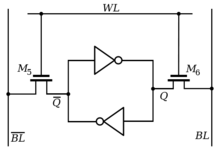
\includegraphics{SRAM.png}
		\caption{SRAM circuit diagram}
	\end{center}
	\end{figure}

\section{DRAM - Dynamic RAM}
DRAM requires a periodic ‘refresh’ of power in order to function. The capacitors that store data in DRAM gradually discharge energy; no energy means the data becomes lost. This is why DRAM is called ‘dynamic’ — constant change or action (e.g. refreshing) is needed to keep data intact. For storing information in this cell, transistor T is turned on and an appropriate voltage is applied to the bit line. This causes a known amount of charge to be stored in the capacitor. After the transistor is turned off, due to the property of the capacitor, it starts to discharge. Hence, the information stored in the cell can be read correctly only if it is read before the charge on the capacitors drops below some threshold value.
\\
\\The advantages of using DRAM (vs. SRAM) are lower costs of manufacturing and greater memory capacities.
\\The disadvantages of using DRAM (vs. SRAM) are slower access speeds and higher power consumption. 
\\Because of these characteristics, DRAM is typically used in:
	\begin{itemize}
		\item System memory
		\item Video graphics memory
	\end{itemize}

	\begin{figure}[H]
	\begin{center}
		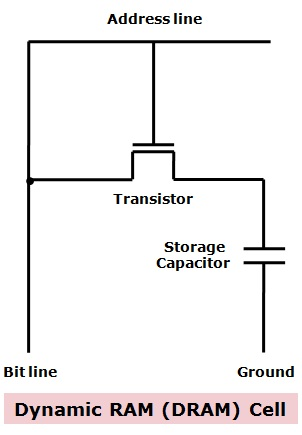
\includegraphics{DRAM.jpg}
		\caption{DRAM circuit diagram}
	\end{center}
	\end{figure}

\section{SDRAM - Synchronous Dynamic RAM or SDR SDRAM - Single Data Rate Synchronous Dynamic RAM}
SDRAM is a classification of DRAM that operates in sync with the CPU clock, which means that it waits for the clock signal before responding to data input whereas DRAM is asynchronous, \ie responds to input immediately. Allowing synchronisation helps the CPU to process overlapping instructions in parallel, \ie pipelining. Pipeling helps in processing more instructions simultaneously, leading to faster transfer/peformance rates. It fetches the read or write instruction during the rising edge of the clock of the CPU.
\\
\\The advantage of SDR SDRAM is that it allows pipelining. 

\section{DDR SDRAM - Double Data Rate Synchronous Dynamic RAM}
DDR SDRAM operates like SDR SDRAM but can fetch the read or write instruction during the rising as well as the falling edge of the clock, and hence the name, 'Double data rate', allowing for twice as many instructions being performed. There are multiple generations in the DDR SDRAM. which are DDR2, DDR3, DDR4. The improvements are along the lines of advanced signal processing, greater memory capacity, lower memory consumption(upto 1.2 V) and higher standard clock speeds (upto 1600 MHz).
\\
\\The advantage of DDR SDRAM is that it allows faster rates (double that of SDR SDRAM) of processing instructions.

\section{GDDR SDRAM - Graphics Double Data Rate Synchronous Dynamic RAM}
GDDR SDRAM is a type of DDR SDRAM that is specifically designed for video graphics rendering, typically in conjunction with a dedicated GPU (graphics processing unit) on a video card. It has multiple generations too, which are GDDR2, GDDR3, GDDR4, GDDR5 which include improving performance and lowering power consumption. Despite sharing similar properties with DDR SDRAM, it is very different. GDDR favours bandwith over latency, since its expected to process enormous amounts of data, not at faster speeds necessarily.
\\
\\The advantage of GDDR SDRAM is that it has higher bandwith.
\\The disadvantage is that it has higher latency.
\end{document}

